\id{IRSTI 65.59.15}

\begin{articleheader}
\sectionwithauthors{T. Tultabayeva, K.Makangali, G. Tokysheva, A. Shoman, D. Aiken}{POTENTIAL OF CHICKEN PROCESSING BY-PRODUCTS IN COLLAGEN PROTEIN
HYDROLYSATE PRODUCTION BASED ON DISTAL LIMBS AND STOMACHS}

T. Tultabayeva\textsuperscript{\envelope }, K.Makangali, G. Tokysheva, A. Shoman,
D. Aiken
\end{articleheader}

\begin{affiliation}
NJSC «S.Seifullin Kazakh agrotechnical research University», Astana,
Kazakhstan

\raggedright {\bfseries \textsuperscript{\envelope }}Corresponding-author: \href{mailto:tultabayeva@inbox.ru}{\nolinkurl{tultabayeva@inbox.ru}}
\end{affiliation}

This study investigates the feasibility of producing collagen protein
hydrolysates from chicken processing by-products, specifically distal
limbs and stomachs, which are often treated as waste in the poultry
industry. With the increasing demand for sustainable and functional
ingredients, these by-products offer a valuable source of bioactive
proteins, including collagen, that can be transformed into protein
hydrolysates for use in the food industry. The research evaluates key
physical and chemical properties, including water-binding capacity,
shear stress, viscosity, and protein digestibility, to determine the
suitability of distal limbs and stomachs for hydrolysate production.
Using structural analysis, we measured the mechanical resistance and
structural stability of these by-products, with findings showing that
distal limbs have a high collagen content (11.3\%) and excellent water
retention, while stomachs exhibit lower fat content (2.1\%) and high
protein concentration (21.4\%), making both suitable for hydrolysis.
Viscosity and shear stress tests further support the use of these
materials, indicating stability and strong structural integrity under
processing conditions. Additionally, protein digestibility studies
suggest that collagen hydrolysates from these sources may have enhanced
bioavailability. The results suggest that utilizing distal limbs and
stomachs for collagen hydrolysate production is a viable approach to
create functional, high-protein food ingredients while also addressing
sustainability by reducing waste. By transforming these by-products, the
poultry industry can contribute to circular economy practices, enhance
resource efficiency, and promote eco-friendly food production. This
research underscores the potential for incorporating collagen protein
hydrolysates from poultry by-products into various food applications,
presenting both economic and environmental benefits.

{\bfseries Keywords:} poultry by-products, sustainable food production,
collagen protein hydrolysates, chicken stomachs, physicochemical
properties.

ПОТЕНЦИАЛ ПОБОЧНЫХ ПРОДУКТОВ ПЕРЕРАБОТКИ ПТИЦЫ ДЛЯ

\begin{articleheader}
{\bfseries ПРОИЗВОДСТВА БЕЛКОВЫХ КОЛЛАГЕНОВЫХ ГИДРОЛИЗАТОВ НА ОСНОВЕ
ДИСТАЛЬНЫХ КОНЕЧНОСТЕЙ И ЖЕЛУДКОВ}

Т.Ч. Тултабаева\textsuperscript{\envelope }, К.К. Макангали, Г.М. Токышева, А.Е.
Шоман, Д.К. Айкен
\end{articleheader}

\begin{affiliation}
НАО «Казахский агротехнический исследовательский университет
им.С.Сейфуллина»,

Астана, Казахстан,

e-mail: \href{mailto:tultabayeva@inbox.ru}{\nolinkurl{tultabayeva@inbox.ru}}
\end{affiliation}

В данном исследовании изучается возможность производства коллагеновых
белковых гидролизатов из побочных продуктов переработки курицы, в
частности из дистальных конечностей и желудков, которые часто
рассматриваются как отходы в птицеводческой отрасли. С ростом спроса на
устойчивые и функциональные ингредиенты эти побочные продукты
представляют собой ценный источник биоактивных белков, включая коллаген,
которые могут быть превращены в белковые гидролизаты для использования в
пищевой промышленности. В работе оцениваются ключевые физико- химические
свойства, такие как влагосвязывающая способность, напряжение сдвига,
вязкость и усвояемость белков, чтобы определить пригодность дистальных
конечностей и желудков для производства гидролизатов.

С использованием структурного анализа были проведены измерения
механической прочности и структурной стабильности побочных продуктов.
Результаты показали, что дистальные конечности обладают высоким
содержанием коллагена (11,3\%) и отличной способностью удерживать влагу,
в то время как желудки имеют низкое содержание жира (2,1\%) и высокую
концентрацию белка (21,4\%), что делает оба материала подходящими для
гидролиза. Испытания на вязкость и напряжение сдвига дополнительно
подтвердили стабильность и высокую структурную целостность этих
материалов в условиях обработки. Более того, исследования усвояемости
белка показали, что коллагеновые гидролизаты из этих источников могут
обладать улучшенной биодоступностью. Полученные результаты
свидетельствуют о том, что использование дистальных конечностей и
желудков для производства коллагеновых гидролизатов является
перспективным подходом для создания функциональных, высокобелковых
пищевых ингредиентов, а также способствует устойчивому развитию за счет
сокращения отходов. Преобразуя эти побочные продукты, птицеводческая
отрасль может внести вклад в практики циркулярной экономики, повысить
эффективность использования ресурсов и поддержать экологически чистое
производство. Данное исследование подчеркивает потенциал включения
коллагеновых белковых гидролизатов из побочных продуктов птицеводства в
различные пищевые продукты, предлагая как экономические, так и
экологические преимущества.

{\bfseries Ключевые слова:} побочные продукты птицеводства, устойчивое
производство продуктов питания, коллагеновые белковые гидролизаты,
куриные желудки, физико- химические свойства.

\begin{articleheader}
{\bfseries ҚҰС ӨҢДЕУ ҚАЛДЫҚТАРЫНЫҢ ДИСТАЛЬДЫ АЯҚТАР МЕН АСҚАЗАНДАР НЕГІЗІНДЕ
КОЛЛАГЕНДІ АҚУЫЗ ГИДРОЛИЗАТЫН ӨНДІРУДЕГІ ӘЛЕУЕТІ}

{\bfseries Т.Ч. Тултабаева\textsuperscript{\envelope }, Қ.Қ. Мақанғали, Г.М.
Токышева, А.Е. Шоман, Д.К. Айкен}
\end{articleheader}

\begin{affiliation}
«С.Сейфуллина атындағы Қазақ агротехникалық зерттеу университеті» КеАҚ,
Астана қ.,

Қазақстан Республикасы,

e-mail: \href{mailto:tultabayeva@inbox.ru}{\nolinkurl{tultabayeva@inbox.ru}}
\end{affiliation}

Бұл зерттеу тауық өңдеу қалдықтарынан, атап айтқанда дистальды аяқтар
мен асқазандардан, коллагенді ақуыз гидролизаттарын өндіру мүмкіндігін
зерттейді, себебі олар құс шаруашылығында жиі қалдық ретінде
қарастырылады. Тұрақты және функционалды ингредиенттерге деген
сұраныстың артуына байланысты, бұл қалдықтар биологиялық белсенді
ақуыздардың, соның ішінде коллагеннің, құнды көзі болып табылады және
оларды тағам өнеркәсібінде қолдануға арналған ақуыз гидролизаттарына
айналдыруға болады. Зерттеу гидролизат өндірісіне жарамдылығын анықтау
үшін су ұстау қабілеті, кесу кернеуі, тұтқырлық және ақуыздың
сіңімділігі сияқты негізгі физикалық және химиялық қасиеттерін
бағалайды. Құрылымдық талдау арқылы біз бұл қалдықтардың механикалық
беріктігі мен құрылымдық тұрақтылығын өлшедік; нәтижелер көрсеткендей,
дистальды аяқтарда коллагеннің жоғары мөлшері (11,3\%) және суды жақсы
ұстай алу қабілеті бар, ал асқазандардың майы аз (2,1\%) және ақуыз
концентрациясы жоғары (21,4\%), бұл екеуін де гидролизге қолайлы етеді.
Тұтқырлық пен кесу кернеуіне жасалған сынақтар бұл материалдардың өңдеу
жағдайларында тұрақтылығын және құрылымдық тұтастығын растайды. Қосымша
ақуыз сіңімділігіне жасалған зерттеулер осы көздерден алынған коллаген
гидролизаттарының биожетімділігінің жоғары болатынын көрсетеді.
Нәтижелер бойынша дистальды аяқтар мен асқазандарды коллаген
гидролизатын өндіруде пайдалану қалдықтарды азайта отырып, функционалды,
ақуызға бай тағамдық ингредиенттер жасау үшін тиімді тәсіл болып
табылады. Бұл қалдықтарды өңдеу арқылы құс шаруашылығы айналмалы
экономикаға үлес қосып, ресурстарды тиімді пайдаланып, экологиялық таза
тағам өндірісін қолдай алады. Бұл зерттеу құс шаруашылығындағы
қалдықтардан алынған

коллаген гидролизаттарын әртүрлі тағам қолданбаларына енгізу әлеуетін
көрсетеді және оның экономикалық әрі экологиялық пайдасын атап
көрсетеді.

{\bfseries Түйін сөздер:} құс өңдеу қалдықтары, тұрақты азық-түлік
өндірісі, коллагенді ақуыз гидролизаттары, тауық асқазандары,
физика-химиялық қасиеттер.

\begin{multicols}{2}
{\bfseries Introduction.} Poultry farms play an essential role in modern
agriculture, providing the population with vital food products, such as
meat and eggs. These products are highly valued for their nutritional
content, accessibility, and versatile culinary applications {[}1{]}.
Poultry farms are capable of producing high-quality products with
relatively minimal labor and resource inputs compared to other livestock
sectors {[}2{]}. Poultry production is instrumental in ensuring food
security, representing the fastest-growing segment of animal husbandry
in many countries {[}3{]}, with egg and poultry meat production meeting
the needs of both rural and urban populations {[}4{]}. The production of
eggs and poultry meat contributes to economic growth by generating
employment opportunities across large enterprises and small to
medium-sized farms {[}5{]} and supports smallholder operations that
supply local communities with food {[}6{]}. In developed countries,
poultry farming is leveraged to address national food security
objectives by increasing the supply of valuable food resources like meat
and eggs {[}7{]}. Beyond food provision, poultry farming is a critical
tool in combating poverty and improving living standards in rural areas.
In developing countries, poultry serves as an essential asset for
impoverished households, providing income and food security {[}8{]}.
Poultry production also promotes sustainable agricultural development by
enabling efficient resource use and enhancing food security {[}9{]}.
With the rising demand for poultry products, such as meat and eggs, many
countries, including those still developing, face challenges in securing
adequate resources for the sector {[}10{]}. Issues include environmental
pollution due to waste and the consumption of natural resources for
poultry feed {[}11{]}. However, in response to these challenges, many
nations are working to develop more sustainable farming practices aimed
at reducing environmental impacts {[}12{]}. Thus, poultry farms have a
significant impact on food provision, economic development, and the
improvement of living standards through job creation and enhanced food
security.

In Kazakhstan, the poultry sector occupies a central position within
animal husbandry, playing a crucial role in providing the population
with socially significant food products, including poultry meat and
eggs. Currently, the country has 69 poultry farms, comprising 34 for egg
production, 29 for meat production, and 6 breeding farms. Additionally,
Kazakhstan is expanding the capacity of four poultry farms to produce an
additional 200,000 tons of poultry meat per year, which will satisfy
domestic poultry meat demand and support export potential, as reported
by the Prime Minister' s press service {[}13{]}.
Specifically, the following farms will be funded: Canadian Chicken
Limited in Akmola Region with an annual output of 12,500 tons, Alel Agro
in Zhambyl Region with 25,000 tons, Prima Kus in Almaty Region with
35,000 tons, and Aitas KZ in Almaty Region with 120,000 tons. The
projects will be financed by the Development Bank of Kazakhstan and
implemented between 2025 and 2026. This indicates a sustained increase
in production and processing costs, underscoring the need for process
optimization and efficiency improvements in the poultry sector, along
with exploring innovative ways to reduce production costs, including
through secondary raw material utilization.

The objective of this study is to examine the secondary raw materials
from poultry processing to justify their application in the production
of protein hydrolysates.

{\bfseries Materials and methods.} The subjects of this study encompassed
chicken distal limbs and stomachs. Shear stress and viscosity of the
meat raw material were meticulously assessed using the Structurometer
ST2 (Lab Quality LLC, Russia) to analyze the mechanical properties of
sausage products, such as shear resistance and viscosity.

Shear force measurements were conducted with the Structurometer ST2,
which recorded force values F upon application to the sausage sample.
Cross-sectional area A was quantified by measuring the blade-sample
contact surface.

Shear rate γ was derived from sample characteristics and experimental
conditions, with structurometer-generated data employed to calculate
viscosity, providing insights into the raw material's resistance to
deformation under shear load.

Water activity in the sausage products was evaluated using the Aqualab
4TE device (METER Group, USA), while chemical composition of the meat
materials was precisely determined using the TANGO R spectrometer
(Bruker, Germany), equipped with a pre-loaded calibration model to
ensure accurate compositional analysis.

{\bfseries Results and discussion.} The experiments were conducted using
the Structurometer ST2 (manufactured by Labreactive, Russia), with all
measurements performed in six replicates. To determine shear stress, the
force and deformation of the meat samples were evaluated (Figures 1 and
2).
\end{multicols}

\begin{figure}[H]
	\centering
	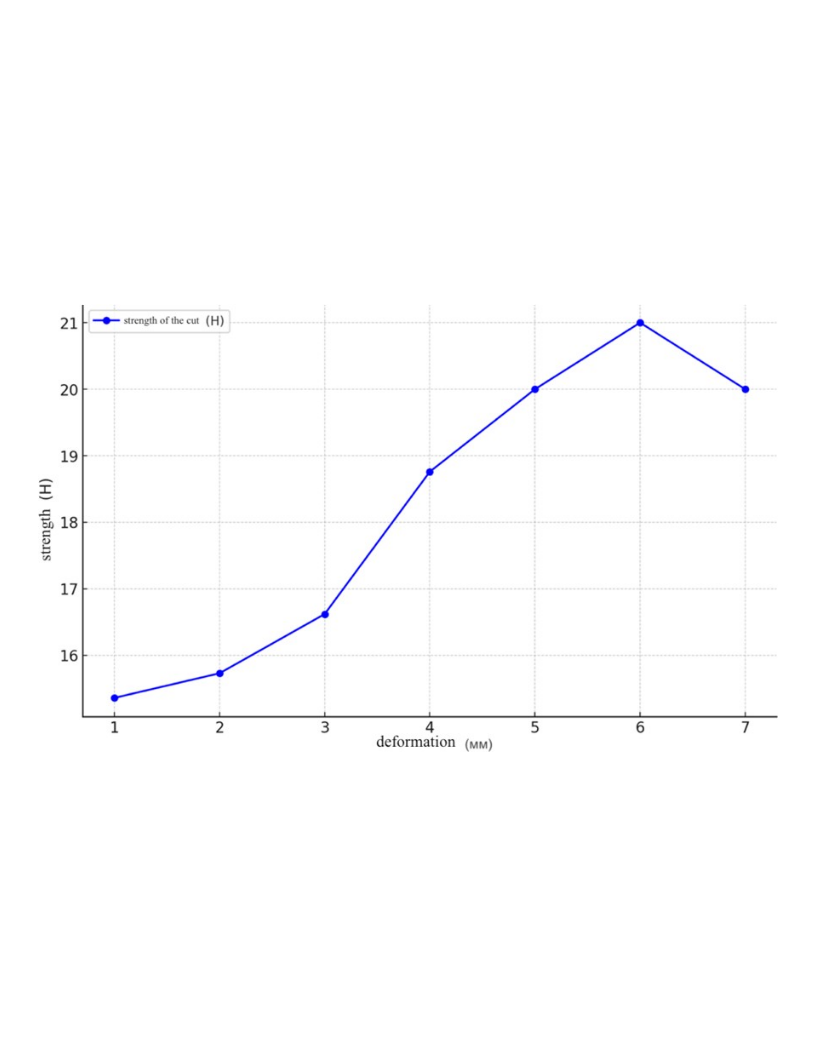
\includegraphics[width=0.7\textwidth]{media/pish/image9}
	\caption*{Figure 1 - Shear Force of Chicken Distal Limbs}
\end{figure}

\begin{multicols}{2}
At the initial stage (1--2 mm), the shear force gradually increases,
starting from approximately 16 N. Between 3--5 mm of deformation, a more
substantial increase in shear force is observed, reaching 20 N. The
maximum shear force (21 N) is recorded at around 6 mm of deformation.
Following this, at 7 mm of deformation, the shear force slightly
decreases to just above 20 N.
\end{multicols}

\begin{figure}[H]
	\centering
	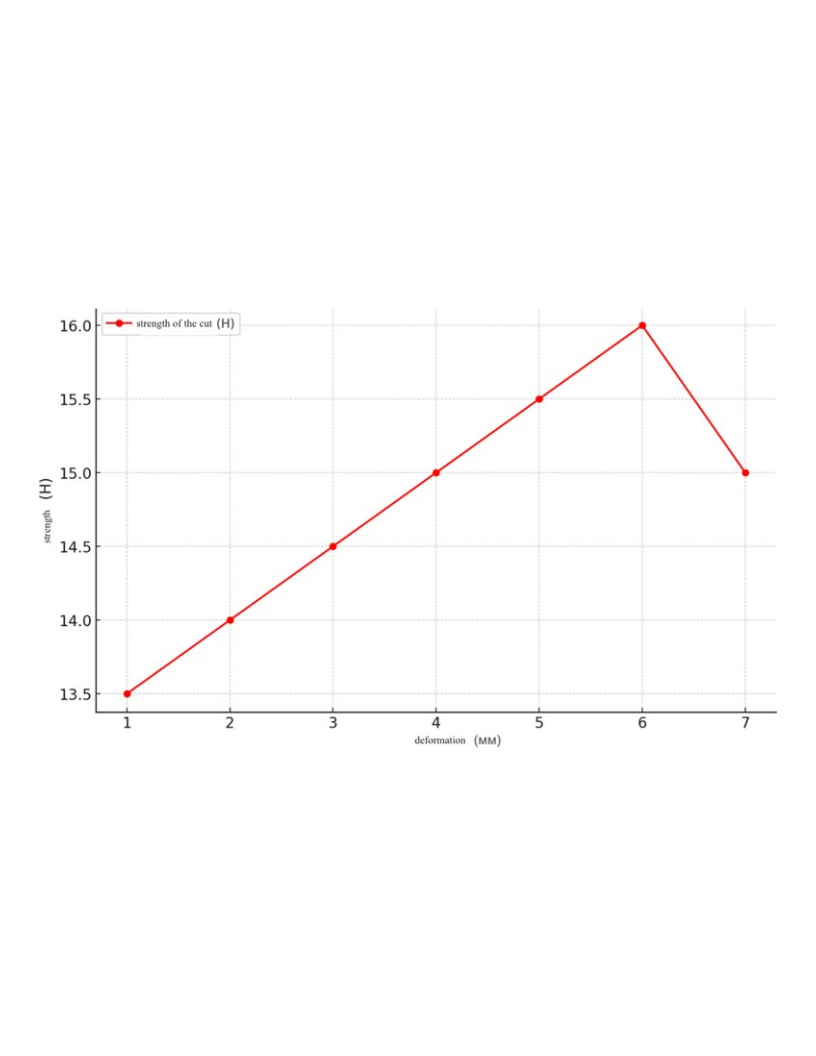
\includegraphics[width=0.65\textwidth]{media/pish/image10}
	\caption*{Figure 2 - Shear Force of Chicken Stomachs}
\end{figure}

\begin{multicols}{2}
At the initial stage (1--2 mm), the shear force of chicken stomachs
starts at around 13.5 N and gradually increases. From 3 to 5 mm, a
linear increase in shear force is observed, reaching approximately 15.5
N. The maximum shear force is recorded at 6 mm of deformation, measuring
around 16 N. Beyond this point, at 7 mm of deformation, the shear force
decreases to 15 N.

Based on the obtained data on shear force, deformation, and shear rate,
the shear stress and viscosity of the meat raw material were determined
(Figure 3).
\end{multicols}

\begin{figure}[H]
	\centering
	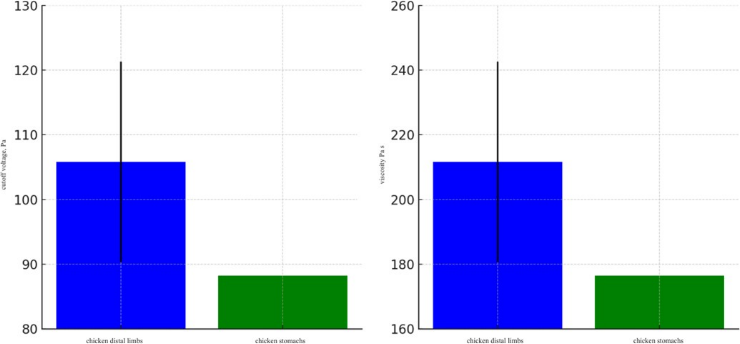
\includegraphics[width=0.65\textwidth]{media/pish/image11}
	\caption*{Figure 3 -Shear Stress and Viscosity of Meat Raw Material}
\end{figure}

\begin{multicols}{2}
The shear stress for chicken distal limbs reaches approximately 110 Pa,
indicating high mechanical strength and structural stability of this raw
material. The shear stress for chicken stomachs is somewhat lower,
around 90 Pa, which also reflects robust structures suitable for further
processing. The viscosity of chicken distal limbs is approximately 220
Pa·s, indicating a high capacity for retaining moisture and fats, an
essential characteristic for hydrolysate production. The viscosity of
chicken stomachs is lower, around 180 Pa·s, which is also an acceptable
value for collagen extraction processes.

study of water-binding capacity (WBC) of chicken limbs and stomachs
further allows for an assessment of their potential as collagen sources.
Collagen-rich limbs and stomachs demonstrate a high capacity to retain
water, which can significantly enhance the texture and stability of
hydrolysates (fig.4).
\end{multicols}

\begin{figure}[H]
	\centering
	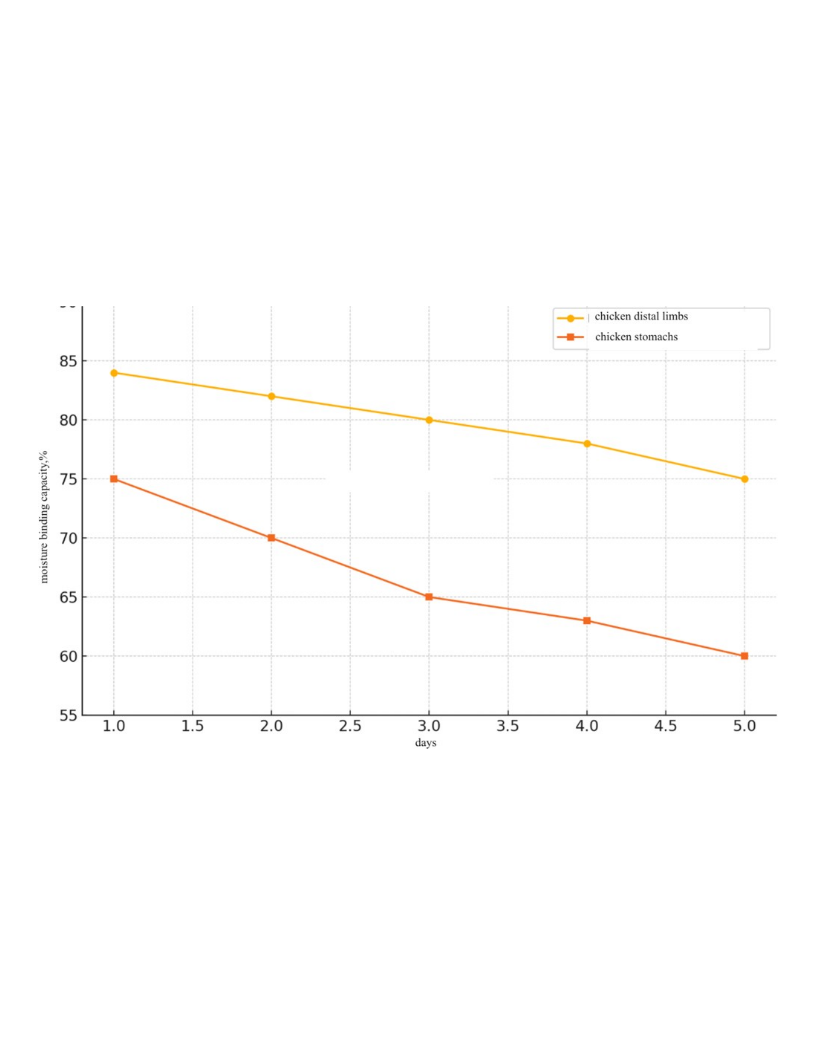
\includegraphics[width=0.6\textwidth]{media/pish/image12}
	\caption*{Figure 4 -- Changes in Water-Binding Capacity (WBC) of Meat Raw
Material Over 5 Days}
\end{figure}

\begin{multicols}{2}
The water-binding capacity (WBC) of chicken distal limbs (yellow line)
starts at around

85\% on the first day and gradually decreases to 80\% by the fifth day,
indicating relatively high moisture retention stability over the study
period. The WBC of chicken stomachs (orange line) is initially lower,
about 75\% on the first day, and continues to decrease to approximately
65\% by the fifth day.

For successful collagen hydrolysate production, the initial
physicochemical properties of the raw material, such as moisture
content, water activity, and pH, play a crucial role (Table 1).
\end{multicols}

\begin{table}[H]
\caption*{Table 1 -- Physicochemical Properties of Meat Raw Material}
\centering
\begin{tabular}{|l|l|l|}
\hline
Indicators & Storage, days & Chicken Distal Limbs \\ \hline
Moisture, \% &
  \begin{tabular}[c]{@{}l@{}}1 days\\ 3 days\\ 6 days\\ 9 days\end{tabular} &
  \begin{tabular}[c]{@{}l@{}}65,42 ± 0,06\\ 59,1 ± 0,11\\ 57,6 ± 0,12\\ 57,2 ± 0,12\end{tabular} \\ \hline
Active Acidity, pH &
  \begin{tabular}[c]{@{}l@{}}1 days\\ 3 days\\ 6 days\\ 9 days\end{tabular} &
  \begin{tabular}[c]{@{}l@{}}6,17 ± 0,12\\ 6,19 ± 0,09\\ 6,25 ± 0,05\\ 6,24 ± 0,06\end{tabular} \\ \hline
Water Activity aw, c.u. &
  \begin{tabular}[c]{@{}l@{}}1 days\\ 3 days\\ 6 days\\ 9 days\end{tabular} &
  \begin{tabular}[c]{@{}l@{}}0,825± 0,003\\ 0,827± 0,002\\ 0,824± 0,000\\ 0,819± 0,002\end{tabular} \\ \hline
\end{tabular}
\end{table}

\begin{multicols}{2}
Chicken distal limbs and stomachs exhibit similar moisture values at
each stage of storage. On the first day, the moisture content of chicken
limbs is 65.42\%, while that of chicken stomachs is 67.34\%. By the
sixth day, these values decrease to 57.6\% and 59.3\%, respectively.
Despite the overall reduction in moisture, both types of raw materials
maintain sufficiently high levels, which is crucial for hydrolysis, as
hydrolysates require a certain moisture level for effective protein
extraction. The slightly higher moisture content in chicken stomachs
potentially makes them more efficient for hydrolysate production,
particularly in scenarios where maximum moisture retention is essential.

A detailed analysis of the chemical composition is crucial to assess the
suitability of various raw materials for collagen hydrolysate
production. The chemical composition determines key parameters such as
protein, collagen, fat, and moisture content, which directly affect the
hydrolysis efficiency and the quality of the final product. Let us
consider the chemical composition of chicken distal limbs and stomachs
to evaluate their potential for further processing and use in protein
hydrolysate production (Table 2).
\end{multicols}

\begin{table}[H]
\caption*{Table 2 -- Chemical Composition of Meat Raw Material}
\centering
\begin{tabular}{|l|l|l|}
\hline
Indicators & Chicken Distal Limbs, \% & Chicken Stomachs, \% \\ \hline
Fat        & 14,6                     & 2,1                  \\ \hline
Protein    & 21,1                     & 21,4                 \\ \hline
Moisture   & 2,3                      & 2,9                  \\ \hline
Collagen   & 11,3                     & 7,5                  \\ \hline
BEFFE      & 17,9                     & 14,7                 \\ \hline
\end{tabular}
\end{table}

\begin{multicols}{2}
Chicken distal limbs contain 14.6\% fat, which is significantly higher
than the 2.1\% fat content found in chicken stomachs. The high fat
content in distal limbs may require additional processing for fat
removal prior to hydrolysis; however, the extracted fat can also be
utilized in other production processes, such as the development of
bioactive components. Stomachs, with their lower fat content, require
less intensive preparation, simplifying the hydrolysis process.

{\bfseries Conclusion.} The results of the study confirm the high
suitability of chicken distal limbs and stomachs for processing into
collagen protein hydrolysates. The chemical composition of

these raw materials highlights key components that make them promising
for applications across various industries. Specifically, chicken distal
limbs contain 11.3\% collagen, significantly higher than the 7.5\% in
chicken stomachs, indicating their substantial value for
collagen-containing products. Additionally, distal limbs exhibit a
higher BEFFE (17.9\% versus 14.7\% in stomachs), suggesting better
protein extractability, which is beneficial for hydrolysis processes.
Chicken stomachs, despite having a lower collagen content, offer notable
advantages, such as low fat content (2.1\% compared to 14.6\% in limbs)
and high protein concentration (21.4\%), making them ideal for processes
that require minimal fat. This simplifies the pre-treatment of raw
materials before hydrolysis, allowing efficient use in protein product
manufacturing. Thus, processing chicken distal limbs and stomachs for
collagen hydrolysate production represents an economically viable and
environmentally sustainable approach to utilizing poultry slaughter by-
products.

\emph{{\bfseries Financing.} This research is funded by the Ministry of
Agriculture of the Republic of Kazakhstan (BR24892775)}
\end{multicols}

\begin{center}
{\bfseries References}
\end{center}

\begin{references}
\begin{enumerate}
\def\labelenumi{\arabic{enumi}.}
\item
  Luchkin, A., Lukasheva, O., Novikova, N., Zyatkova, A., \& Yarotskaya,
  E. (2021). Feasibility study of the influence of the diet on the
  quality characteristics of poultry production. IOP Conference Series:
  Earth and Environmental Science, 640. DOI
  10.1088/1755-1315/640/3/032041.
\item
  Pica-Ciamarra, U., \& Otte, J. (2010). Poultry, food security and
  poverty in India: looking beyond the farm-gate.
  World' s Poultry Science Journal, 66, 309 - 320. DOI
  10.1017/S0043933910000358.
\end{enumerate}

3.Akinola, L., \& Essien, A. (2011). Relevance of rural poultry
production in developing countries with special reference to Africa.
World' s Poultry Science Journal, 67, 697 - 705.

DOI 10.1017/S0043933911000778.

4.Mead G. C. Poultry meat processing and quality. -- Cambridge: Woodhead
Publishing Limited, 2004. -- 400 p. ISBN I 85573 727 2

5.Baker, R., \& Passmore, D.Role of Poultry \& Egg Production in the
Economy of the United
States.//\href{https://www.researchgate.net/journal/SSRN-Electronic-Journal-1556-5068?_tp=eyJjb250ZXh0Ijp7ImZpcnN0UGFnZSI6InB1YmxpY2F0aW9uIiwicGFnZSI6InB1YmxpY2F0aW9uIn19}{SSRN
Electronic Journal}.-2010.- DOI 10.2139/SSRN.1581500.

6.Pankova, S., \& Katerinich, O. Efficiency of using the new domestic
meat-egg hybrid for the production of food eggs in household farms//
\href{https://agrisp.com/index.php/agrisp/issue/view/11}{Agricultural
Science and Practice}.-2017.- Vol. 4(2).- P.47-51. DOI
10.15407/agrisp4.02.047.

7.Efremova, A. (2018). Role of Poultry Industry in public food supply//
Economic Sciences for Agribusiness and Rural Economy.- 2018.-Vol. 2.- S.
29-36. DOI 10.22630/esare.2018.2.2.

8.Sonaiya, E. (2007). Family poultry, food security and the impact of
HPAI. //World' s Poultry Science Journal.- 2207.-
Vol.63(1).-P. 132 - 138. DOI 10.1017/S0043933907001353.

9.Gunnarsson, S., Segerkvist, K., Göransson, L., Hansson, H., \&
Sonesson, U. (2020). Systematic Mapping of Research on Farm-Level
Sustainability in Egg and Chicken Meat Production//
Sustainability.-2020-Vol. 12(7), 3033. DOI 10.3390/su12073033.

10.Mottet, A., \& Tempio, G. (2017). Global poultry production: current
state and future outlook and challenges// World' s
Poultry Science Journal/-Vol. 73,.-P.245 - 256.

DOI 10.1017/S0043933917000071.

11. Karkach, P., Mashkin, Y., \& Fesenko, V. (2023). Environmental
problems of industrial and organic poultry farming// Tehnologìâ
virobnictva ì pererobki produktìv tvarinnictva.-2023.-Vol.1.-
P.145-158.DOI 10.33245/2310-9289-2023-178-1-145-158. {[} in Ukrainian{]}

12. Laca, A., Laca, A., \& Díaz, M. (2021). Environmental impact of
poultry farming and egg
production// \href{https://www.sciencedirect.com/book/9780128213636/environmental-impact-of-agro-food-industry-and-food-consumption}{Environmental
Impact of Agro-Food Industry and Food Consumption}.-2021.-P.81-100.

\href{https://doi.org/10.1016/B978-0-12-821363-6.00010-2}{DOI
10.1016/B978-0-12-821363-6.00010-2}.

13.Oficial' nyj informacionnyj resurs
Prem' er-ministra Respubliki Kazahstan URL:\\
\href{https://primeminister.kz/ru/news/investitsii-v-apk-pozvolyat-za-2-goda-polnostyu-
zakryt-potrebnost-v-myase-ptitsy-i-nachat-eksport-28485/}{https://primeminister.kz} {[}in Russian{]}
\end{references}

\begin{authorinfo}
\hspace{1em}\emph{{\bfseries Information about the authors}}

Tultabayeva T. - Doctor of Technical Sciences, Associate Professor,
Kazakh Agrotechnical Research University named after S.Seifullin,
Astana, Kazakhstan, e-mail:
\href{mailto:tultabayeva@inbox.ru}{\nolinkurl{tultabayeva@inbox.ru}};

Makangali K. -- PhD, Kazakh Agrotechnical Research University named
after S.Seifullin, Astana, Kazakhstan, e-mail:\\
\href{mailto:kmakangali@mail.ru}{\nolinkurl{kmakangali@mail.ru}};

Tokysheva G. - PhD, Kazakh Agrotechnical Research University named after
S.Seifullin, Astana, Kazakhstan, e-mail:\\
\href{mailto:tokisheva_g@mail.ru}{\nolinkurl{tokisheva\_g@mail.ru}};

Shoman A. - PhD, Kazakh Agrotechnical Research University named after
S.Seifullin, Astana, Kazakhstan, e-mail:
\href{mailto:shoman_aruzhan@mail.ru}{\nolinkurl{shoman\_aruzhan@mail.ru}};

Aiken D. {\bfseries -} Master of Technical Sciences, Kazakh Agrotechnical
Research University named after S.Seifullin, Astana, Kazakhstan, e-mail:
\href{mailto:didi_dom@mail.ru}{\nolinkurl{didi\_dom@mail.ru}}.

\hspace{1em}\emph{{\bfseries Сведения об авторах}}

Тултабаева Т.Ч. -- д.т.н., доцент, Казахский агротехнический
исследовательский университет им.С.Сейфуллина, Астана, Казахстан,
e-mail:
\href{mailto:tultabayeva@inbox.ru}{\nolinkurl{tultabayeva@inbox.ru}};

Макангали К.К. - PhD, Казахский агротехнический исследовательский
университет им.С.Сейфуллина, Астана, Казахстан, e-mail:
\href{mailto:kmakangali@mail.ru}{\nolinkurl{kmakangali@mail.ru}};

Токышева Г.М. - PhD, Казахский агротехнический исследовательский
университет им.С.Сейфуллина, Астана, Казахстан, e-mail:
\href{mailto:tokisheva_g@mail.ru}{\nolinkurl{tokisheva\_g@mail.ru}};

Шоман А.Е. - PhD, Казахский агротехнический исследовательский
университет им. С.Сейфуллина, Астана, Казахстан, e-mail:
\href{mailto:shoman_aruzhan@mail.ru}{\nolinkurl{shoman\_aruzhan@mail.ru}};

Айкен Д.К. -- м.т.н., Казахский агротехнический исследовательский
университет им.С.Сейфуллина, Астана, Казахстан, e-mail:
\href{mailto:didi_dom@mail.ru}{\nolinkurl{didi\_dom@mail.ru}}.
\end{authorinfo}
